For the \ac{nn} approach, first an assignment matrix as the one depicted in \cref{fig:assignM} is built. Observations that are know within the gate of a certain track, will be identified as $X$. Otherwise, the distance function of of the corresponding observation and track is calculated. 

\begin{figure}[h]
	\centering
	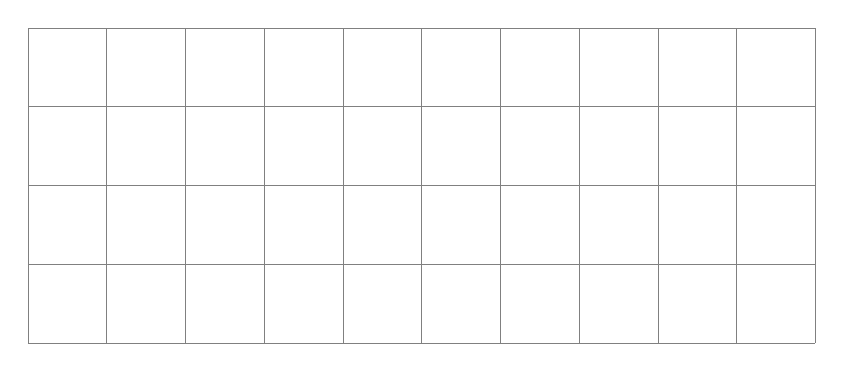
\begin{tikzpicture}
% Reference Grid
\draw[gray,very thin] (0,0) grid (10,4); 

\end{tikzpicture}
	\caption{Assignment matrix example}
	\label{fig:assignM}
\end{figure} 

There are different ways to solve the assignment problem from the assignment matrix following a \ac{nn}-approach.Two suboptimal solutions are presented and (LATER: OPTIMAL SOLUTION).

Suboptimal Solution one:
\begin{enumerate}
	\item Observations that are considered for singly-validated tracks will not be considered for mutiply-validated tracks. 
	\item Observations that are in multiple tracks will not be considered for tracks that contain single-validated observations
	\item Repeat 1. and 2. until the assignment matrix is not changed anymore 
	\item For the remaining tracks with multiple observations, select the observation with minimum distance 
	\item For the remaining observations that validate with various tracks, assign to th track with the minimum distance
\end{enumerate}

Suboptimal Solution two:
\begin{enumerate}
    \item Search the matrix for the minimum distance observation-to-track pair and assign it
    \item  Remove the assigned pair from the matrix and repeat 1. until all possible assignments have been made. 
\end{enumerate}